\chapter{The compartmental model: end-stage renal disease}
\label{applications-fits_incon_v_con}
\chapterprecis{Sarah K. Wolf, Abraham D. Flaxman, Mohsen Naghavi, and Giuseppe Remuzzi}

We now turn our attention to conditions where systematic review
uncovered a substantial amount of nonprevalence data, which we wish
to use to inform our estimates.  This was already touched on in
chapter~\ref{applications-age_groups} and will be investigated more
systematically in the next few chapters.  We begin by considering
end-stage renal disease (ESRD) treated with dialysis, a condition for which data on
prevalence, incidence, remission, and with-condition mortality were
all collected in relatively large quantities through systematic
review.

ESRD is the final stage of chronic kidney disease (CKD), the slow and
progressive loss of kidney function.  The most common causes of CKD
are diabetes and high blood pressure.  Damage to kidneys is usually
permanent, but treatment and lifestyle changes can slow disease progression.  However, at the final stage of the disease, the kidneys no longer function,
and the patient needs dialysis or a kidney transplant to survive.
There are two main types of
dialysis for kidney treatment: hemodialysis and peritoneal dialysis.
Hemodialysis filters waste and excess fluids from the blood
externally using a machine, while peritoneal dialysis uses the lining
of the peritoneal cavity and a catheter to filter wastes from the
blood. \cite{_k/doqi_2002, dipiro_pharmacotherapy:_2008}

This example focuses on ESRD treated with dialysis, combining hemodialysis
and peritoneal dialysis for analysis.
Most of the data are from studies or registry reports.
Transplantation incidence among the prevalent
dialysis population was used as a proxy for remission.  The analysis
includes $5664$ data points representing $161$ countries in
all $21$ GBD 2010 regions.  Data from Australasia are shown in
figure~\ref{fig:app-CKD data}.
%%   The distribution of dialysis
%% epidemiological parameter data types by region are shown in Table
%% \ref{tab:CKD_data}.


%% \begin{table}[h]
%%     \begin{center}
%%         \caption{ Frequency of dialysis epidemiological parameter data types by region used in analysis}
%%         \label{tab:CKD_data}
%%         \rowcolors{1}{}{gray!50}
%%         \begin{tabular}{|p{3cm}|c|c|c|p{1.5cm}|c|}
%%             \hline
%%                 Region & Prevalence & Incidence & Remission & \centering With-condition mortality & Total \\
%%             \hline
%%                 \raggedright North America, High Income & 277 & 554 & 241 & \centering 240 & 1312 \\
%%                 \raggedright Europe, Western & 362 & 694 & 65 & \centering 10 & 1131 \\
%%                 \raggedright Australasia & 332 & 403 & 144 & \centering 219 & 1098 \\
%%                 \raggedright Asia Pacific, High Income & 161 & 168 & 16 & \centering 26 & 371 \\
%%                 \raggedright Asia, Southeast & 138 & 131 & 14 & \centering 0 & 283 \\
%%                 \raggedright Latin America, Southern & 112 & 113 & 20 & \centering 0 & 245 \\
%%                 \raggedright Asia, East & 107 & 105 & 7 & \centering 0 & 219 \\
%%                 \raggedright Europe, Central & 102 & 86 & 18 & \centering 10 & 216 \\
%%                 \raggedright North Africa Middle East & 76 & 55 & 17 & \centering 2 & 150 \\
%%                 \raggedright Europe, Eastern & 53 & 53 & 13 & \centering 0 & 119 \\
%%                 \raggedright Sub-Saharan Africa, West & 21 & 18 & 51 & \centering 0 & 90 \\
%%                 \raggedright Asia, South  & 35 & 29 & 8 & \centering 0 & 72 \\
%%                 \raggedright Latin America, Tropical & 42 & 10 & 6 & \centering 6 & 64 \\
%%                 \raggedright Sub-Saharan Africa, East & 12 & 9 & 39 & \centering 0 & 60 \\
%%                 \raggedright Latin America, Central & 24 & 21 & 12 & \centering 1 & 58 \\
%%                 \raggedright Caribbean & 15 & 9 & 33 & \centering 0 & 57 \\
%%                 \raggedright Oceania & 13 & 13 & 18 & \centering 0 & 44 \\
%%                 \raggedright Sub-Saharan Africa, Central & 9 & 9 & 18 & \centering 0 & 36 \\
%%                 \raggedright Sub-Saharan Africa, Southern & 6 & 2 & 15 & \centering 0 & 23 \\
%%                 \raggedright Asia, Central & 2 & 1 & 6 & \centering 0 & 9 \\
%%                 \raggedright Latin America, Andean & 5 & 2 & 0 & \centering 0 & 7 \\
%%                 \raggedright Total & 1904 & 2485 & 761 & \centering 514 & 5664 \\
%%             \hline
%%         \end{tabular}
%%     \end{center}
%% \end{table}

    \begin{figure}[h]
        \begin{center}
            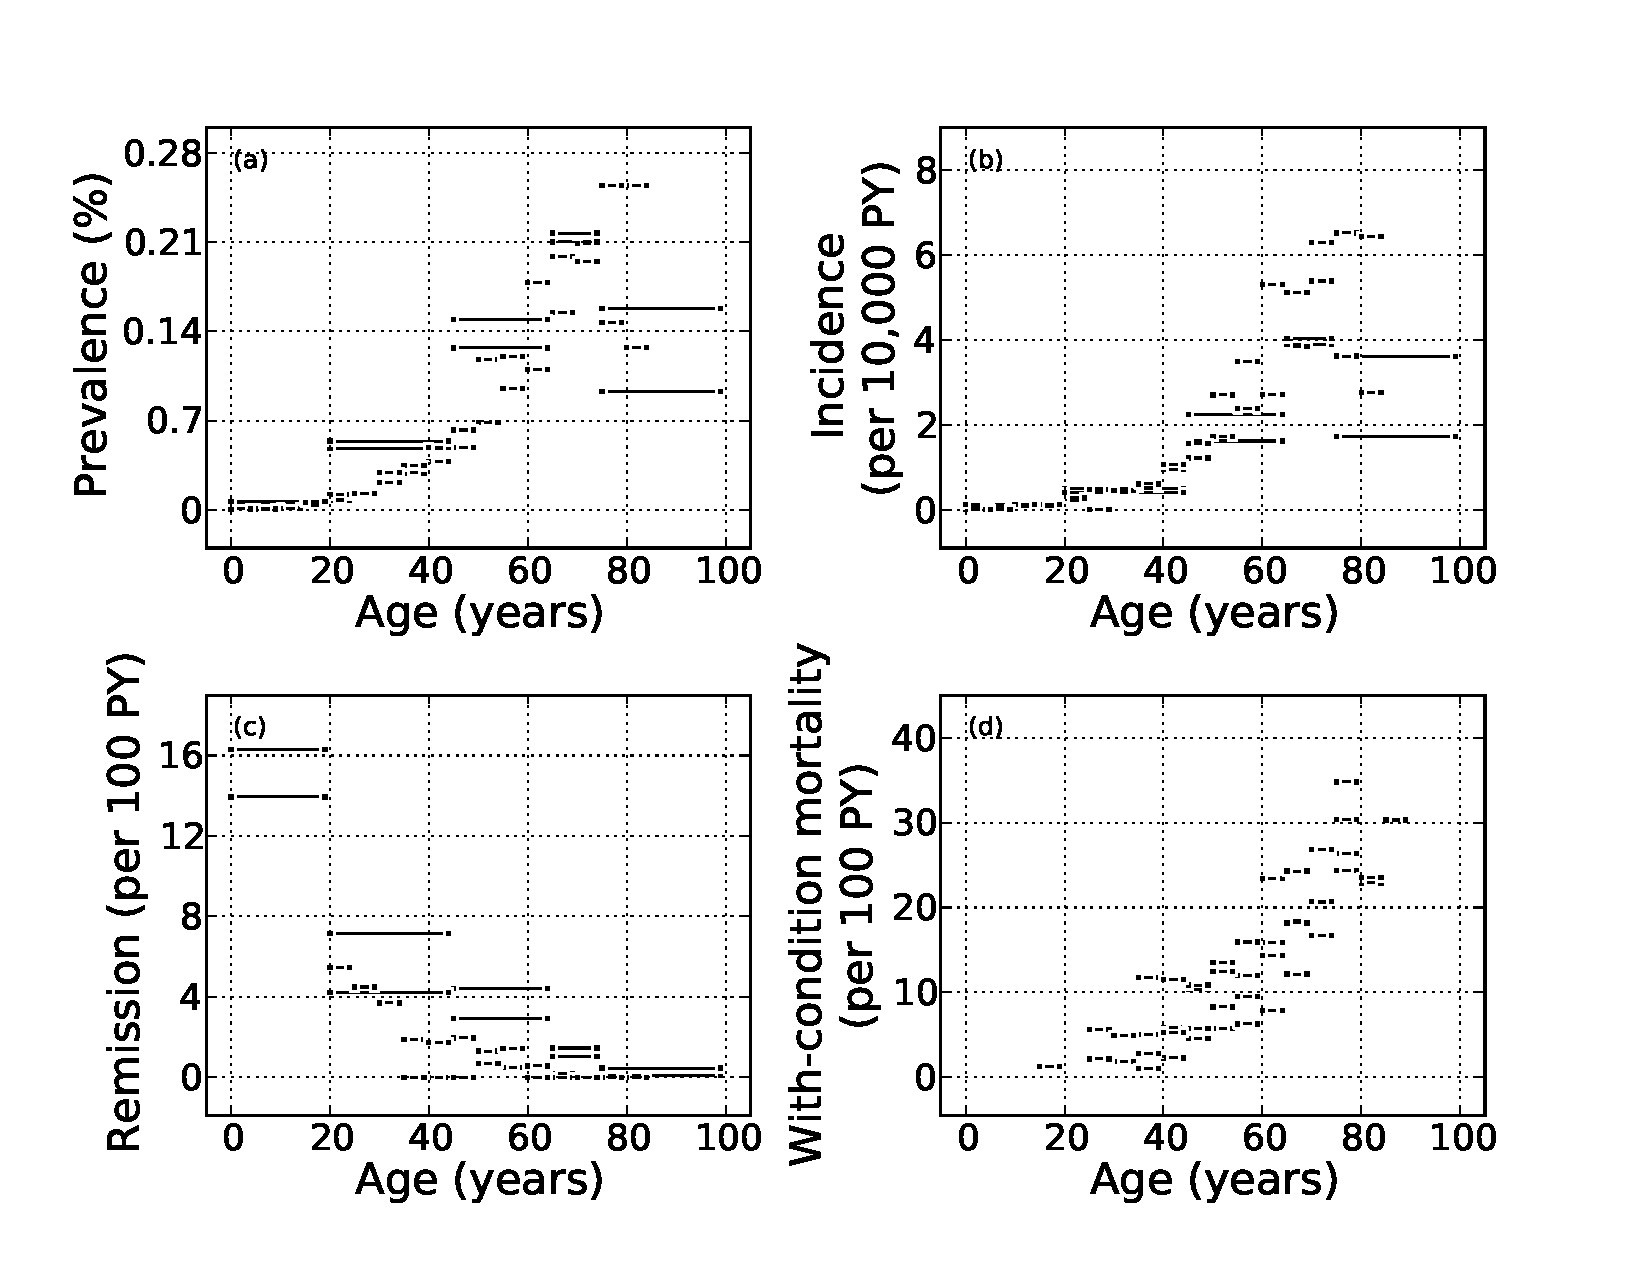
\includegraphics[width=\textwidth]{ckd-data.pdf}
            \caption[Systematic review data for end-stage renal disease
              treated with dialysis.]{Four types of data for Australasian
              males with ESRD treated with dialysis
              in 2005: (a) prevalence, (b) incidence, (c)
              remission, and (d) with-condition mortality.}
            \label{fig:app-CKD data}
        \end{center}
    \end{figure}

As discussed in section~\ref{sys-dynamics}, epidemiological parameters,
such as incidence, prevalence, remission, and with-condition
mortality, are related by a logical requirement of internal
consistency.  A prevalent case can exist only if there was a past
incident event, and the current number of prevalent cases can be
determined from past prevalent cases, newly incident cases, deaths, and
remissions.  Modeling the parameters simultaneously produces a best
estimate and plausible uncertainty bounds for incidence and prevalence
that are internally consistent for a single time, place, and sex.

Figure~\ref{fig:app-CKD incon v con} compares the compartmental and
spline model results for Australasian males with
ESRD treated with dialysis in 2005.  While the spline model estimates each
epidemiological parameter individually, the compartmental model estimates
prevalence, incidence, remission, and with-condition mortality
simultaneously.  Figure~\ref{fig:app-CKD incon v con} and a
comparison of the age-standardized prevalence estimates for the region
show that the compartmental model estimates do not follow the data
like the spline model does.  As seen in figure~\ref{fig:app-CKD asp}, the
spline model produces prevalence estimates that are systematically lower
than those of the compartmental model because of the logic requirement that
requires all prevalent cases to have a corresponding incident event.

    \begin{figure}[h]
        \begin{center}
            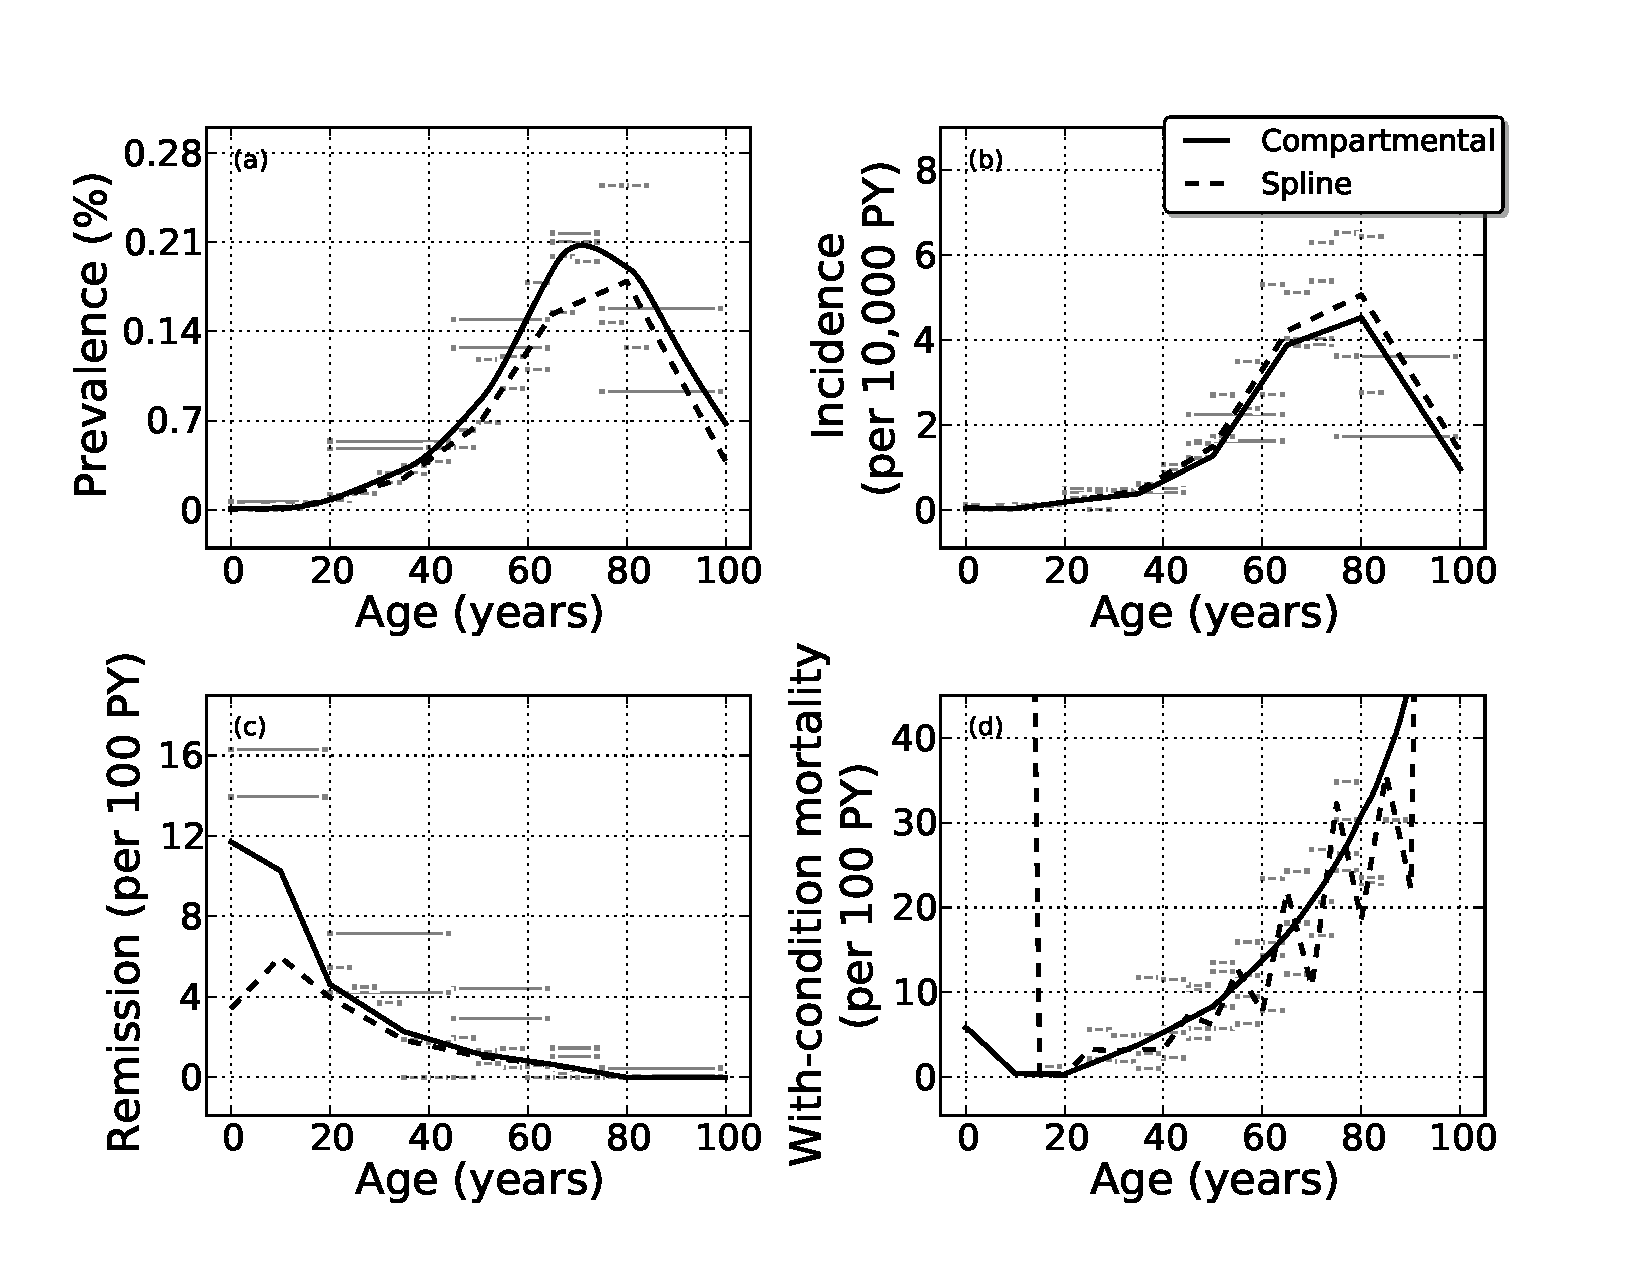
\includegraphics[width=\textwidth]{ckd-incon_v_con.pdf}
            \caption[Comparison of epidemiological parameter estimates for
              end-stage renal disease treated with dialysis using the compartmental and spline models.]{Comparison of epidemiological parameter estimates
              for Australasian males with ESRD treated with dialysis
              in 2005 using the compartmental and spline models.}
            \label{fig:app-CKD incon v con}
        \end{center}
    \end{figure}

    \begin{figure}[h]
        \begin{center}
            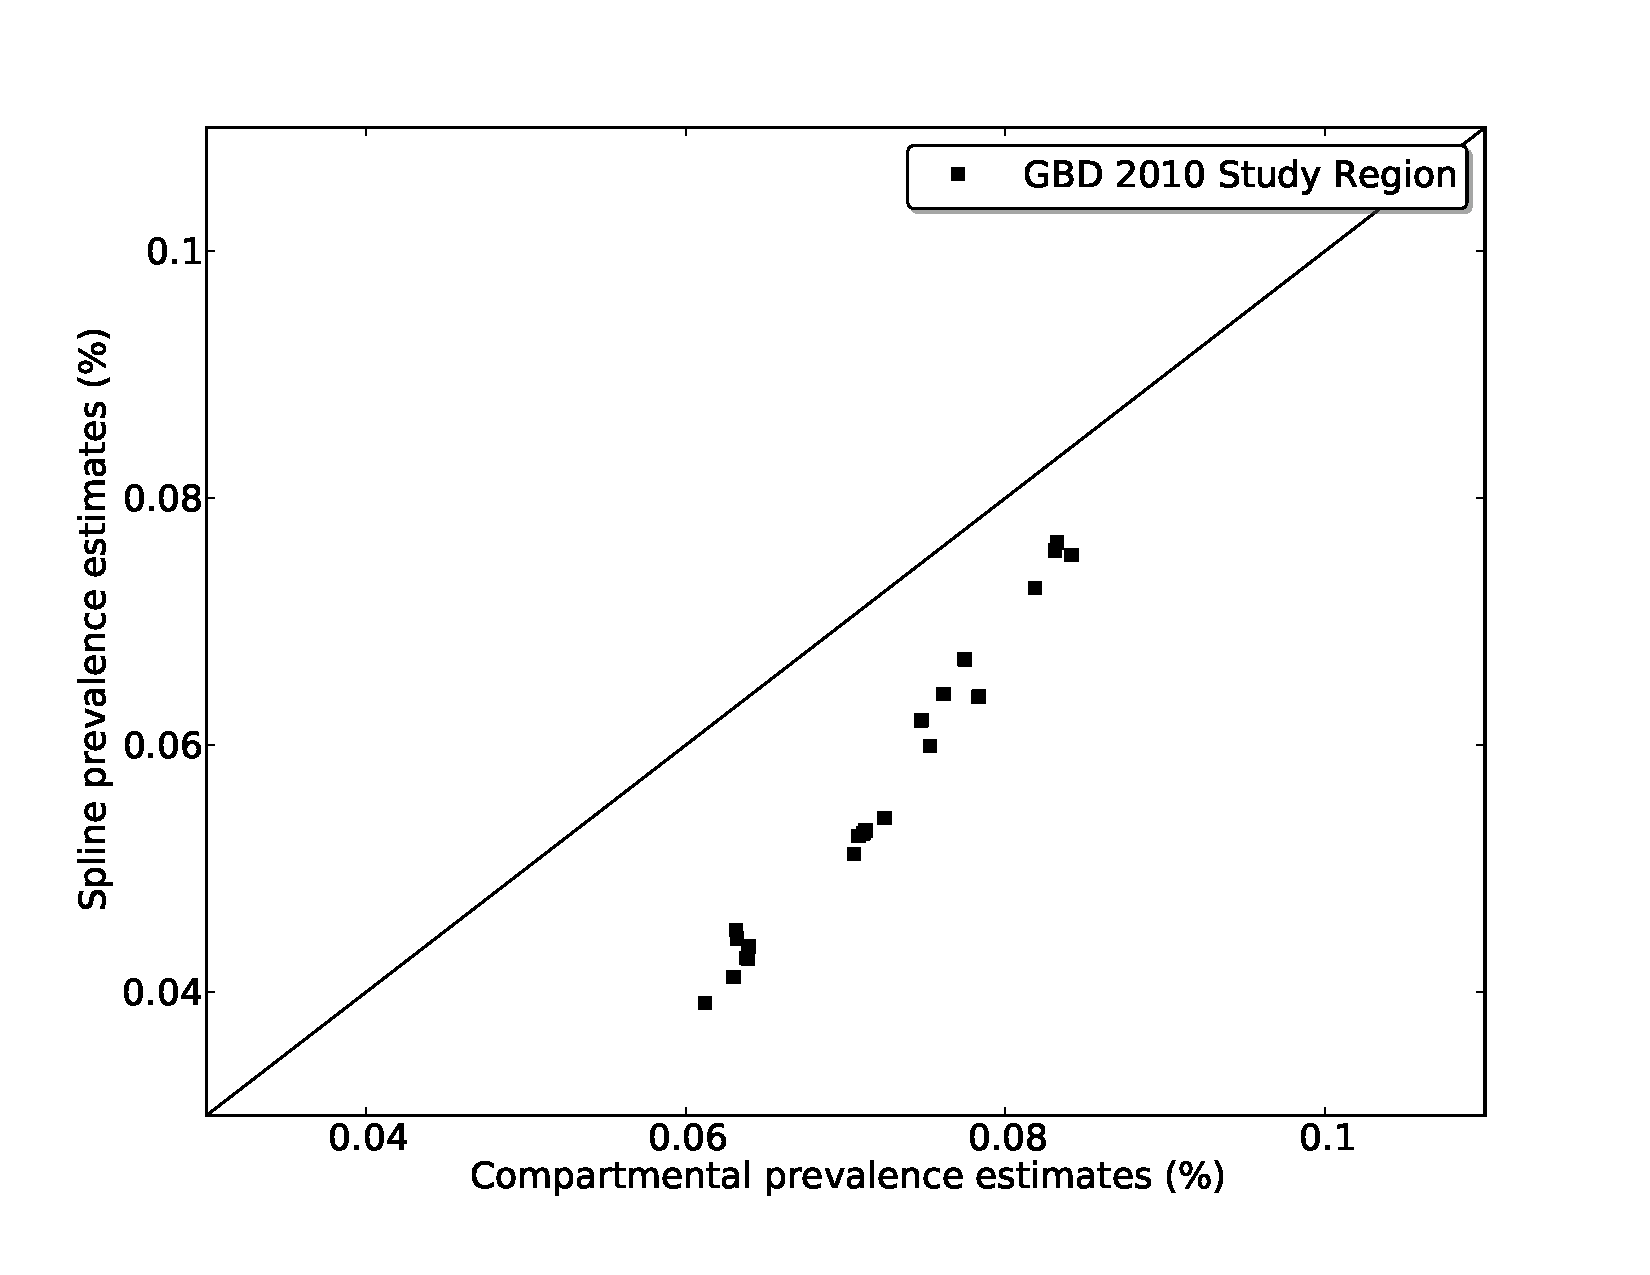
\includegraphics[width=\textwidth]{ckd-asp_scatter.pdf}
            \caption[Comparison of the regional age-standardized
              prevalence estimates using compartmental and spline
              models for end-stage renal disease treated with dialysis.]
              {Comparison of the regional age-standardized
              prevalence estimates using compartmental and spline
              models for males with ESRD treated with dialysis in
              2005.}
            \label{fig:app-CKD asp}
        \end{center}
    \end{figure}

Another advantage to compartmental modeling is an estimate with a smooth
age pattern. Modeling each epidemiological parameter individually, the
spline model follows the data exactly, often producing an
uneven age pattern as seen in figure~\ref{fig:app-CKD smooth}.  This
effect can be minimized by placing an informative prior on the
penalized spline model as discussed in chapter~\ref{theory-age_pattern_model}.

    \begin{figure}[h]
        \begin{center}
            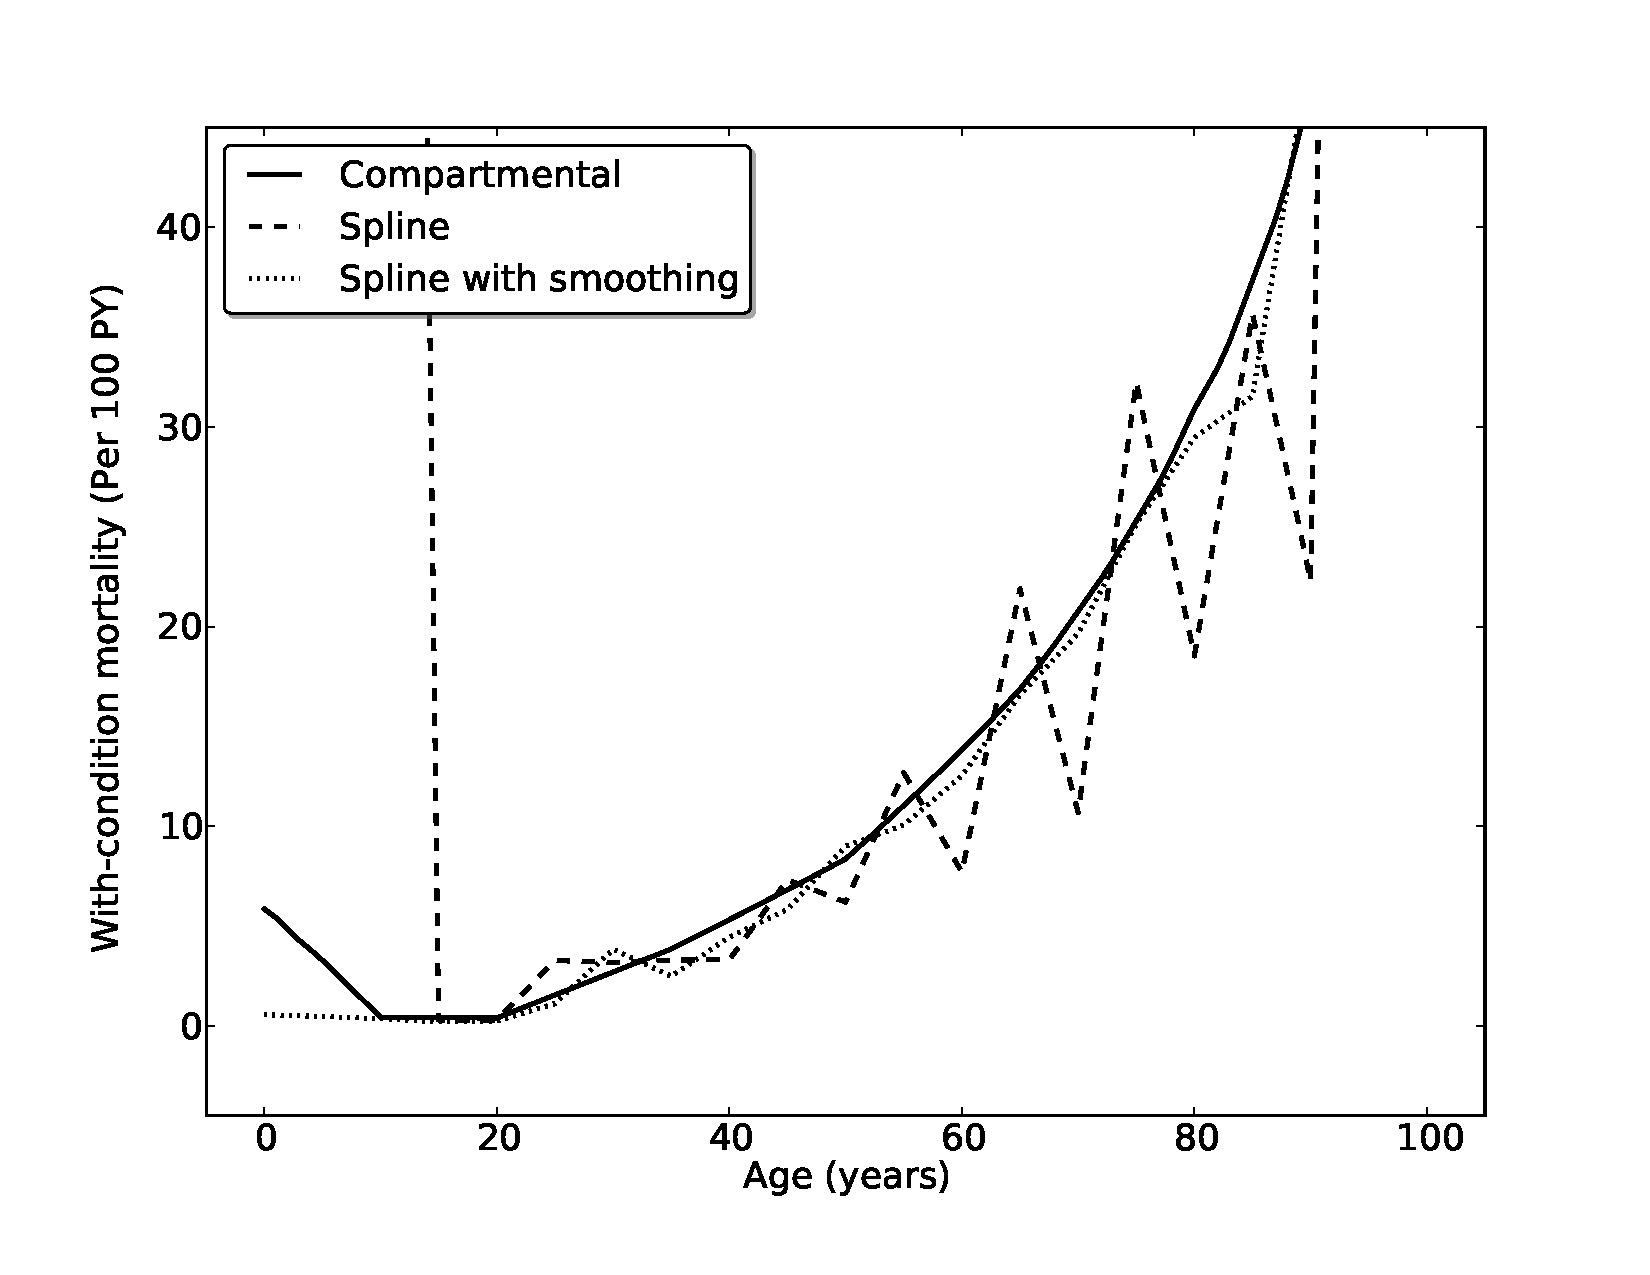
\includegraphics[width=\textwidth]{ckd-m_with_smoothing.pdf}
            \caption[Comparison of with-condition mortality estimates
              for end-stage renal disease treated with dialysis using
              a compartmental model, a spline model, and a spline model
              with a smoothing parameter.]{With-condition mortality estimates for
              Australasian males with ESRD treated with dialysis in
              2005 using a compartmental model, a spline model,
              and a spline model with a smoothing parameter.}
            \label{fig:app-CKD smooth}
        \end{center}
    \end{figure}

The compartmental model is preferable to modeling each parameter
individually with the spline model because it incorporates all
available data.  Simultaneously modeling all data, the compartmental
model produces internally consistent estimates for a single age,
sex, and time.
